% Solar Filament Segmentation Challenge 2026 -- technical report (IEEE conference format, 4 pages).
% Compile on Overleaf with pdfLaTeX (IEEEtran is built in). If the organisers provide their own template, copy the
% body (from \begin{abstract} to the bibliography) into it. Fill in the three macros below before submitting.
\documentclass[conference]{IEEEtran}
\usepackage[utf8]{inputenc}
\usepackage[T1]{fontenc}
\usepackage{amsmath,amssymb}
\usepackage{graphicx}
\usepackage{booktabs}
\usepackage{url}
\usepackage[hidelinks]{hyperref}

\newcommand{\finalLB}{\textbf{[fill in]}}          % public leaderboard score of submission_v3_final.csv
\newcommand{\teamname}{[Kaggle team name]}
\newcommand{\repourl}{\url{https://github.com/umerkang66/solar-filament-segmentation}}

\begin{document}

\title{Solar Filament Instance Segmentation under Annotator Disagreement: Soft Multi-Annotator Targets,
DINOv3 Members and PQ-Additive Instance Selection}

\author{\IEEEauthorblockN{Haseeb Khan and Muhammad Umer}
\IEEEauthorblockA{Team \teamname\\ Affiliation and e-mail: \textit{fill in}}}

\maketitle

\begin{abstract}
We segment solar filaments in $2048\times2048$ GONG H$\alpha$ full-disk images. The metric is Panoptic Quality
(PQ), computed separately against every annotator of an image. Two annotators of the same image agree at only
PQ $=0.340$, so annotator disagreement, not pixel accuracy, limits every honest system. We train U-Net and DINOv3
networks on soft consensus targets. We show that PQ is exactly additive over disjoint predicted instances, and we
use this to tune post-processing and to train instance scorers with nested cross-validation. Our final system
(ResNet-34, EfficientNetV2-S and DINOv3 ConvNeXt-S members, a hypothesis pool with a learned fragment linker and a
stacked scorer) reaches a nested out-of-fold PQ of \textbf{0.4477} on the 707 training images (public leaderboard
\finalLB). We report ceilings, an error breakdown and an analysis of the leaderboard gap.
\end{abstract}

\section{Data}
The training set (MAGFiLO~\cite{magfilo}) has 707 images with 1{,}154 annotation sets and 8{,}199 filament
polygons. 411 images have one annotator, 145 have two and 151 have three. Filaments are thin and elongated (median
area 1{,}228\,px, 5th percentile 317\,px). The 180 test images come from the same six GONG sites and the same years
(2011--2022) in similar proportions. The median gap to the nearest training image is ${\sim}37$\,h, as between
training images, so we treat the test images as a random sample of the same observation pool. Each annotation set
is identified by \texttt{<annotator>-<image>}. The 37 annotator codes (a 4-digit group and a 2-digit slot) have
clearly different styles: from 3.4 to 10.5 polygons per image and a median filament area from 640 to 2{,}100\,px.

\section{Metric analysis}
For every annotation set, all predicted filaments of the image are compared with its ground truth (GT). Pairs with
IoU $>0.5$ are true positives (TP) and contribute their IoU. Counts are pooled over all sets:
PQ $=\sum \mathrm{IoU}_{TP}/(TP+\tfrac12 FP+\tfrac12 FN)$~\cite{kirillov2019panoptic}. Our implementation reproduces
the organisers' notebook exactly.

\textbf{Ceilings.} Table~\ref{tab:ceil} shows that even an oracle that knows every label cannot exceed 0.666 with
one set of masks on multi-annotator images, because the annotators contradict each other. Our system lies above
human consensus because it predicts the average annotator.

\begin{table}[t]
\caption{Human agreement, ceilings and our system (organisers' metric).}\label{tab:ceil}
\centering\footnotesize
\begin{tabular}{@{}lccc@{}}
\toprule
reference & PQ & SQ & RQ \\
\midrule
annotator vs.\ annotator (same image) & 0.340 & 0.634 & 0.536 \\
consensus of two vs.\ held-out third (151 images) & 0.333 & 0.632 & 0.528 \\
oracle with all labels known (296 multi-set images) & 0.666 & 0.825 & 0.807 \\
\textbf{ours} (nested out-of-fold, 707 images) & \textbf{0.448} & 0.683 & 0.655 \\
\bottomrule
\end{tabular}
\end{table}

\textbf{PQ is additive over disjoint instances.} If predicted masks do not overlap, a GT filament can be hit by at
most one prediction. Hence for any subset $S$ of predictions
\begin{equation}
\mathrm{PQ}(S)=\frac{\sum_{i\in S} a_i}{\tfrac12 N_{gt}+\sum_{i\in S} d_i},
\end{equation}
where $a_i$ is the sum of instance $i$'s TP IoUs over the $m_i$ annotation sets of its image and $d_i=m_i/2$.
Adding instance $i$ raises PQ if and only if its expected per-annotator TP IoU $u_i=a_i/m_i$ exceeds PQ$/2$
($\approx0.22$). After extracting instances once, every threshold and filter search is an exact sum. The metric
counts every IoU $>0.5$ pair, so duplicate masks inflate it: submitting each mask twice would raise our
out-of-fold PQ from 0.4385 to 0.4831. \textbf{We submit strictly disjoint masks.}

\section{Method}
\textbf{Targets.} Polygons are rasterised exactly like the GT (pycocotools). The soft target of a pixel is the
fraction of annotators covering it. We also derive a soft skeleton, a soft core and one instance map per annotation
set. Only the \texttt{segmentation} field is read.

\textbf{Networks} (Table~\ref{tab:members}). All members see the full disk as one channel. The v3 members share a
decoder of GroupNorm/GELU/scSE~\cite{roy2018scse} blocks with a light stride-1/2 detail stem, skeleton and core
heads, and deep supervision. M4 uses a DPT decoder~\cite{ranftl2021dpt} on DINOv3 ViT-B/16~\cite{dinov3}.

\begin{table}[t]
\caption{Ensemble members. OOF PQ of each member alone, at the default extraction threshold 0.6 (tuned value in
brackets).}\label{tab:members}
\centering\footnotesize
\begin{tabular}{@{}llcc@{}}
\toprule
member & encoder (pretraining) & px & OOF PQ \\
\midrule
r34\_2048 & ResNet-34 (ImageNet), U-Net & 2048 & 0.4331 \\
effv2s\_1536 & EfficientNetV2-S (ImageNet), U-Net & 1536 & 0.4355 \\
M3 & ResNet-34 (ImageNet), U-Net & 1536 & 0.4131 (0.4303) \\
M4 & DINOv3 ViT-B/16, DPT & 1536 & 0.4268 (0.4410) \\
M5 & DINOv3 ConvNeXt-S, U-Net & 1536 & 0.4303 \\
\bottomrule
\end{tabular}
\end{table}

\textbf{Losses.} The first two members use BCE + soft Dice against the soft target. M3--M5 use BCE + the Jaccard
metric loss JML1~\cite{wang2023jml}, which is minimised at $P=y$ for soft labels. They add a blob
loss~\cite{kofler2023blob} over the instances of one sampled annotation set, so that every filament counts
equally as in PQ, plus skeleton/core head losses and deep supervision. A 5-fold proxy ablation (ResNet-34,
1024\,px) with a paired bootstrap gate chose this loss: BCE + soft Dice 0.3861, BCE + JML1 0.3864 (not
significant), full v3 loss \textbf{0.3956} ($+0.0092$, 90\,\% CI $[+0.006,+0.012]$).

\textbf{Training.} AdamW, warm-up and cosine decay, batch 8, bf16, weight EMA (0.998), 60--80 epochs. DINOv3
encoders use a lower encoder learning rate with layer-wise decay. Images are sampled in proportion to their number
of annotation sets, as the metric weights them. Augmentation runs on the GPU: rotation, flips, scale, shift,
gamma, contrast, blur and noise.

\textbf{Validation.} 5 image-level folds, so all annotation sets of an image share a fold. Every learned
post-processing stage is \emph{nested}: for fold $k$ it is trained on the other folds' out-of-fold predictions.

\textbf{Instances.} Maps are averaged over 8 dihedral TTA views and the 5 fold models of each member, then over
the members. Seeds are the components of $p>t$. Seeds within ${\sim}16$\,px are grouped into one filament, because
annotators draw one polygon around a broken filament ($+0.008$ PQ). The extent is grown by watershed, with holes
filled. The v3-loss members produce softer maps (mean foreground probability 0.80 vs.\ 0.90), so their best
threshold is 0.4 rather than 0.6 (Table~\ref{tab:members}).

\textbf{Selection.} (i) A LightGBM~\cite{ke2017lightgbm} rescorer regresses $u_i$ from 26 instance features and
keeps $u_i>t$; the tuned $t$ matches the theoretical PQ$/2$. (ii) An extent selector picks one of four threshold
levels per filament. (iii) Stage C, used in the final system, builds a pool of hypotheses: threshold families and
a learned fragment linker at two link thresholds. A stacked LightGBM scorer then ranks the candidates, followed by
an overlap-aware greedy selection.

\section{Results}
\begin{table}[t]
\caption{Nested out-of-fold PQ (707 images) and public leaderboard.}\label{tab:results}
\centering\footnotesize
\begin{tabular}{@{}lccc@{}}
\toprule
system & PQ & SQ & LB \\
\midrule
r34 @1024, fixed threshold, no TTA (fold 0) & 0.380 & & \\
+ TTA, tuned thresholds and filters & 0.4205 & & \\
+ rescorer & 0.4272 & & \\
v1: 3-member ensemble + rescorer & 0.4381 & 0.677 & 0.38 \\
v2: r34\_2048 + effv2s\_1536 + extent selector & 0.4438 & 0.680 & 0.38 \\
v2 selector, + M3 & 0.4449 & 0.682 & 0.38 \\
v2 selector, + M5 & 0.4455 & & \\
\textbf{final: Stage C, r34\_2048 + effv2s\_1536 + M5} & \textbf{0.4477} & 0.683 & \finalLB \\
\bottomrule
\end{tabular}
\end{table}

Table~\ref{tab:results} shows the progression. Per-fold validation PQ (single model, no TTA): M3 0.367--0.392, M4
0.385--0.406, M5 0.371--0.412, so the DINOv3 networks are the strongest single members. The selection stages add
little: rescorer $+0.007$, extent selector $+0.0004$ to $+0.003$, Stage C $+0.0022$ over the selector on the final
members. Their oracles show 3--8 points of headroom, but which extent a given annotator draws is largely
unpredictable from the image.

\begin{figure*}[t]
\centering
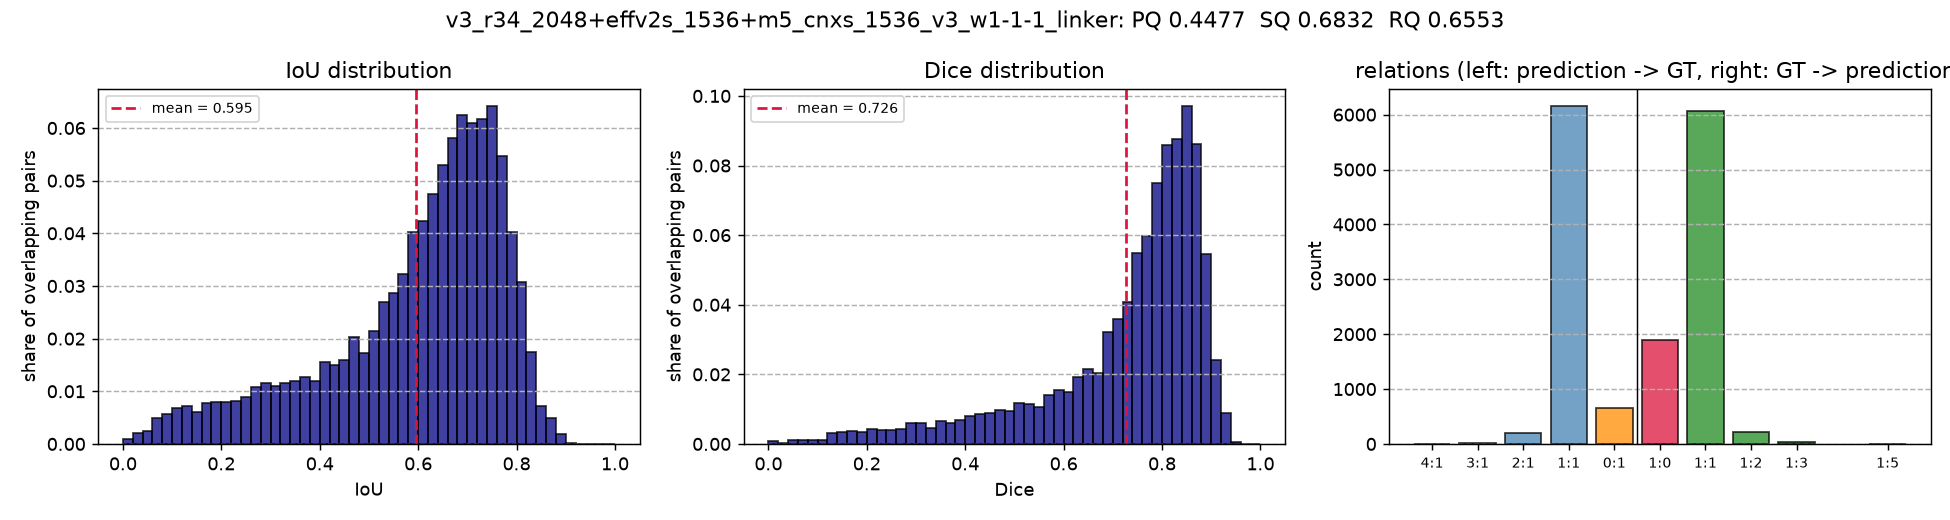
\includegraphics[width=\textwidth]{figures/rubric_final.png}
\caption{Final system, out-of-fold: IoU and Dice distributions of overlapping prediction--GT pairs, and the
relations between predictions and GT filaments (1:1 dominates; 1:$n$ and $n$:1 are rare).}\label{fig:rubric}
\end{figure*}

\textbf{Rubric metrics} (Fig.~\ref{fig:rubric}). 75.7\,\% of overlapping pairs have IoU $>0.5$. The mean/median
IoU is 0.595/0.646 and the mean/median Dice 0.726/0.785. Fragmentation (GT filaments overlapped by 2+ predictions)
is 3.0\,\% and over-merging (predictions overlapping 2+ GT filaments) 2.9\,\%.

\textbf{Where PQ is lost.} 56\,\% of the lost PQ comes from the IoU deficit of true positives (boundary
disagreement), 15\,\% from missed filaments, 14\,\% from wrong extent (IoU $\le0.5$), 6\,\% from spurious
predictions and 10\,\% from fragments and merges. Small filaments are the weakest group ($<500$\,px: PQ 0.29,
recall 0.36), followed by the limb ($r/R>0.8$: PQ 0.37). PQ is uniform across sites (0.43--0.45) and across the
number of annotators per image (0.44/0.46/0.44). It is \emph{not} uniform across annotator groups (0.40--0.55).

\textbf{Leaderboard gap.} Our submissions score 0.38 publicly, ${\sim}0.06$ below out-of-fold, and other teams
report the same gap. It is not chance: random 90-image subsets of our out-of-fold predictions have SD 0.012 and fall
to $\le0.385$ with probability $<0.0003$. It is not mask width: the same masks eroded/dilated by 1\,px score
0.37/0.35. It is not calibration: test maps differ from out-of-fold maps by ${\sim}1$\,\% in foreground fraction.
The most likely cause is an annotator shift, since our PQ varies by 0.15 between annotator groups. We tuned nothing
on the leaderboard.

\textbf{What did not work.} Keeping only the largest component (undoes the $+0.008$ of fragment grouping),
per-instance closing ($-0.003$ to
$-0.016$), multi-scale TTA ($+0.0006$) and JML1 alone ($+0.0003$) were not adopted. Blend weights searched at the v1
threshold 0.6 excluded M4, the best single member; tuning the threshold per blend fixes this. Not run because of
the compute budget: semi-supervised training on unlabelled GONG frames and ConvNeXt-L/ViT-L members.

\section{Compliance, efficiency and reproducibility}
At inference the model sees only the test image. Of the GT fields, only \texttt{segmentation} is used. The public
MAGFiLO v1.0 Kaggle dataset contains 139 of the 180 test images with labels; it was \emph{never downloaded or used}.
No other external data were used, and masks are disjoint. Pretrained weights: ImageNet and DINOv3 (DINOv3 License;
our fine-tuned DINOv3 checkpoints are released with the licence text).

On one AMD Instinct MI300X, training 5 folds $\times$ 60 epochs takes 1.3\,h (M3, 3 folds in parallel), 5.1\,h (M5)
and 6.0\,h (M4). Inference with 8 TTA views takes 0.46--0.72\,s per image and fold model. Post-processing and
selection for 180 test images take 7\,s on 12 CPU workers.

Code, configurations, logs and the reproduction notebook are at \repourl. The final file is reproduced from the
released weights by \texttt{submission\_package\_v3/notebook/reproduce\_v3.ipynb}. Training: \texttt{SETUP.md},
\texttt{scripts/run\_all\_v3.sh}; decisions: \texttt{DECISIONS.md}.

\section*{Acknowledgment}
This work uses DINOv3 (Meta) pretrained weights under the DINOv3 License, and GONG H$\alpha$ data from the NSO
Integrated Synoptic Program (MAGFiLO dataset).

\begin{thebibliography}{10}
\bibitem{magfilo} Earth-Space AI Research Lab, ``MAGFiLO 1.0: multi-annotator GONG filament dataset (MLEcoFi 2024
Dataset V1.0),'' \url{https://www.esairlab.com}, 2024.
\bibitem{kirillov2019panoptic} A.~Kirillov, K.~He, R.~Girshick, C.~Rother, P.~Doll\'ar, ``Panoptic segmentation,''
in \emph{CVPR}, 2019.
\bibitem{dinov3} O.~Sim\'eoni \emph{et al.}, ``DINOv3,'' \emph{arXiv:2508.10104}, 2025.
\bibitem{ranftl2021dpt} R.~Ranftl, A.~Bochkovskiy, V.~Koltun, ``Vision transformers for dense prediction,'' in
\emph{ICCV}, 2021.
\bibitem{wang2023jml} Z.~Wang, X.~Ning, M.~B.~Blaschko, ``Jaccard metric losses: Optimizing the Jaccard index with
soft labels,'' in \emph{NeurIPS}, 2023.
\bibitem{kofler2023blob} F.~Kofler \emph{et al.}, ``blob loss: Instance imbalance aware loss functions for semantic
segmentation,'' in \emph{IPMI}, 2023.
\bibitem{roy2018scse} A.~G.~Roy, N.~Navab, C.~Wachinger, ``Concurrent spatial and channel squeeze \& excitation in
fully convolutional networks,'' in \emph{MICCAI}, 2018.
\bibitem{ke2017lightgbm} G.~Ke \emph{et al.}, ``LightGBM: A highly efficient gradient boosting decision tree,'' in
\emph{NeurIPS}, 2017.
\end{thebibliography}

\end{document}
